\begin{frame}
  \frametitle{Spalart-Allmaras Turbulence Model in Moltres}
  \begin{block}{\textbf{Why the Spalart-Allmaras Model \cite{spalart_one-equation_1994} for Moltres?}}
    A computationally efficient one-equation model that provides reasonable estimates for wall-bounded
    turbulent flows and is tractable for large problems on small computing clusters.
  \end{block}
  \begin{block}{\textbf{Subobjectives}}
    \textbf{Implementation of a Spalart-Allmaras turbulence model in Moltres}
    \begin{itemize}
      \item Implement a Spalart-Allmaras model in Moltres
      \item Verify and validate the model against reference turbulent flow solutions
    \end{itemize}
  \end{block}
\end{frame}

\begin{frame}
  \frametitle{Spalart-Allmaras Turbulence Model in Moltres}
  \textbf{Spalart-Allmaras Model with Rotation Correction Scheme
  \cite{spalart_one-equation_1994, aupoix_extensions_2003, dacles-mariani_numericalexperimental_1995}}\\
  \\
  Governing equation for the modified dynamic viscosity, $\tilde{\mu}$:
  \begin{multline}
    \rho \frac{\partial\tilde{\mu}}{\partial t} + \rho \mathbf{u}\cdot\nabla\tilde{\mu} = \rho c_{b1}
    \left(1-f_{t2}\right)\tilde{S}\tilde{\mu} + \frac{1}{\sigma}\{\nabla\cdot\left[\left(\mu+
    \tilde{\mu}\right)\nabla\tilde{\mu}\right] + c_{b2}|\nabla\tilde{\mu}|^2\} \\
    - \left(c_{w1}f_w - \frac{c_{b1}}{\kappa^2}f_{t2}\right)\left(\frac{\tilde{\mu}}{d}\right)^2
  \end{multline}
  \begin{align*}
    \shortintertext{where}
      \mu_t &= \tilde{\mu}f_{v1} = \text{turbulent eddy viscosity}, \\
      f_{v1} &= \frac{\chi^3}{\chi^3 + c_{v1}^3}, \\
      \chi &= \frac{\tilde{\mu}}{\mu}.
  \end{align*}
%      \tilde{S} &= \Omega + \frac{\tilde{\nu}}{\kappa^2 d^2} f_{v2}, \\
%      f_{v2} &= 1 - \frac{\chi}{1+\chi f_{v1}}, \\
%      \Omega &= \sqrt{2W_{ij}W_{ij}} = \text{vorticity magnitude}, \\
%      W_{ij} &= \frac{1}{2}\left(\frac{\partial u_i}{\partial x_j} - \frac{\partial u_j}{\partial x_i}
%      \right), \\
%        f_w &= g\left(\frac{1 + c_{w3}^6}{g^6 + c_{w3}^6}\right)^{1/6}, \\
%        g &= r + c_{w2}\left(r^6 - r\right), \\
%        r &= \text{min}\left(\frac{\tilde{\nu}}{\tilde{S}\kappa^2d^2}, 10\right), \\
%        f_{t2} &= c_{t3} \exp{\left(-c_{t4}\chi^2\right)},
%    \end{align*}
%  \shortintertext{and the constants are}
%    \sigma = \frac{2}{3}, \ c_{b1} = 0.1355, \ c_{b2} = 0.622, \ \kappa = 0.41, \
%    c_{w1} = \frac{c_{b1}}{\kappa^2} + \frac{1+c_{b2}}{\sigma}, \nonumber \\
%    c_{w2} = 0.3, \ c_{w3} = 2, \
%    c_{v1} = 7.1, \ c_{t3} = 1.2, \ c_{t4} = 0.5 \ \text{.} \nonumber
\end{frame}

\begin{frame}
  \frametitle{Spalart-Allmaras Turbulence Model in Moltres}
  \begin{block}{\textbf{Model Implementation Details}}
  \begin{itemize}
    \item Built on top of an existing incompressible Navier-Stokes model in MOOSE
    \item Uses Streamline-Upwind/Petrov-Galerkin (SUPG) stabilization scheme for numerical stability
    \item Rotation correction scheme \cite{aupoix_extensions_2003, dacles-mariani_numericalexperimental_1995}
      reduces eddy viscosity in regions of rotational but non-turbulent flow
  \end{itemize}
  \end{block}
  \pause
  \begin{block}{\textbf{Verification \& Validation Tests for the Turbulence Model}}
    \begin{enumerate}
      \item Turbulent Channel Flow Verification Test at Re $\approx 13750$
      \begin{itemize}
        \item Reference results: \gls{DNS} results by Moser et al.\ \cite{moser_direct_1999}
      \end{itemize}
      \item Turbulent Pipe Flow Validation Test at Re $\approx 40000$
      \begin{itemize}
        \item Reference results: Experimental results by Laufer \cite{laufer_structure_1954}
      \end{itemize}
      \item Backward-Facing Step Flow Validation Test
      \begin{itemize}
        \item Reference results: Experimental results by Driver \& Seegmiller \cite{driver_features_1985}
        \& Spalart-Allmaras model results from CFL3D CFD code \cite{krist_cfl3d_1998}
      \end{itemize}
    \end{enumerate}
  \end{block}
\end{frame}

\begin{frame}
  \frametitle{Turbulent Channel Flow Verification Test Results}
  \begin{figure}[htb!]
    \centering
    \begin{subfigure}[b]{0.32\columnwidth}
      \centering
      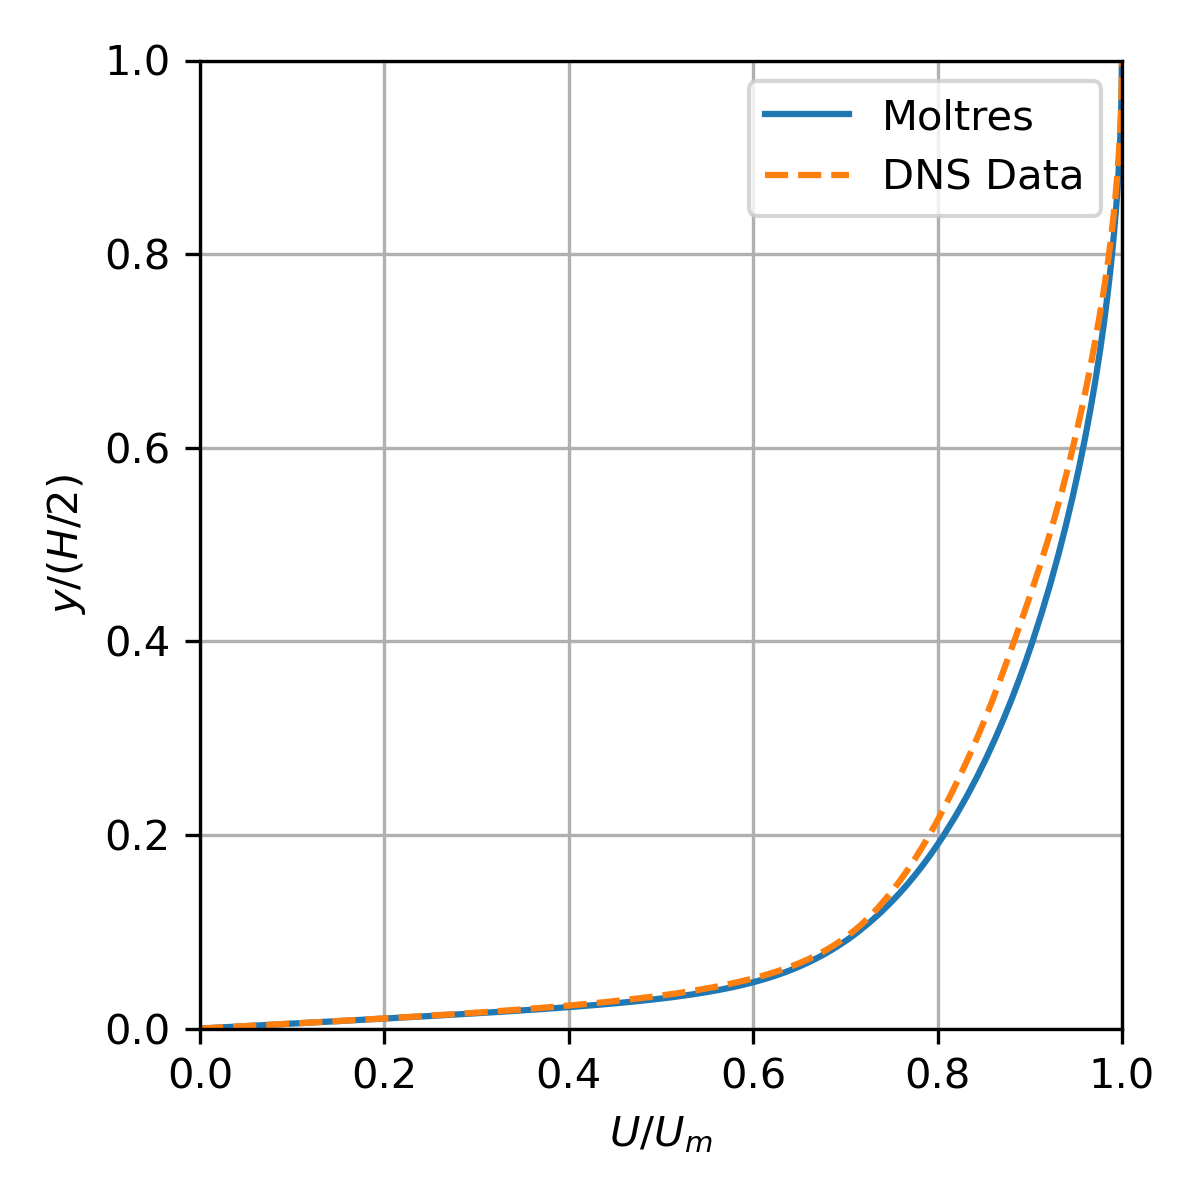
\includegraphics[width=\columnwidth]{channel_vel}
      \caption{Normalized velocity distribution across the channel.}
      \label{fig:channel-vel}
    \end{subfigure}
    \hfill
    \begin{subfigure}[b]{0.32\columnwidth}
      \centering
      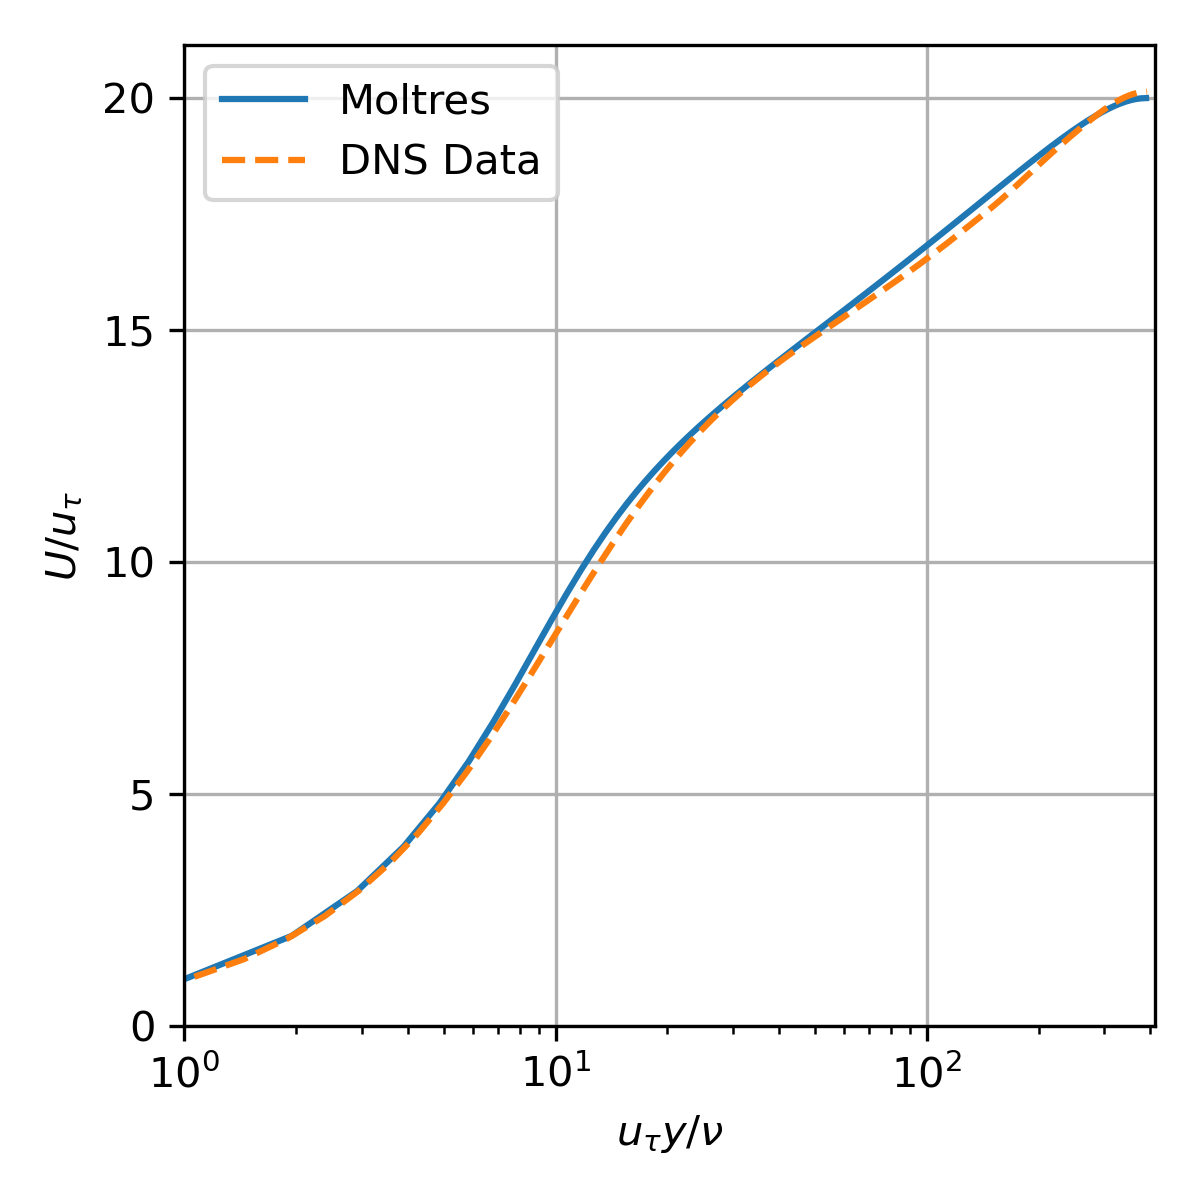
\includegraphics[width=\columnwidth]{channel_nondim}
      \caption{Dimensionless velocity vs.\ dimensionless wall distance.}
      \label{fig:channel-nondim}
    \end{subfigure}
    \begin{subfigure}[b]{0.32\columnwidth}
      \centering
      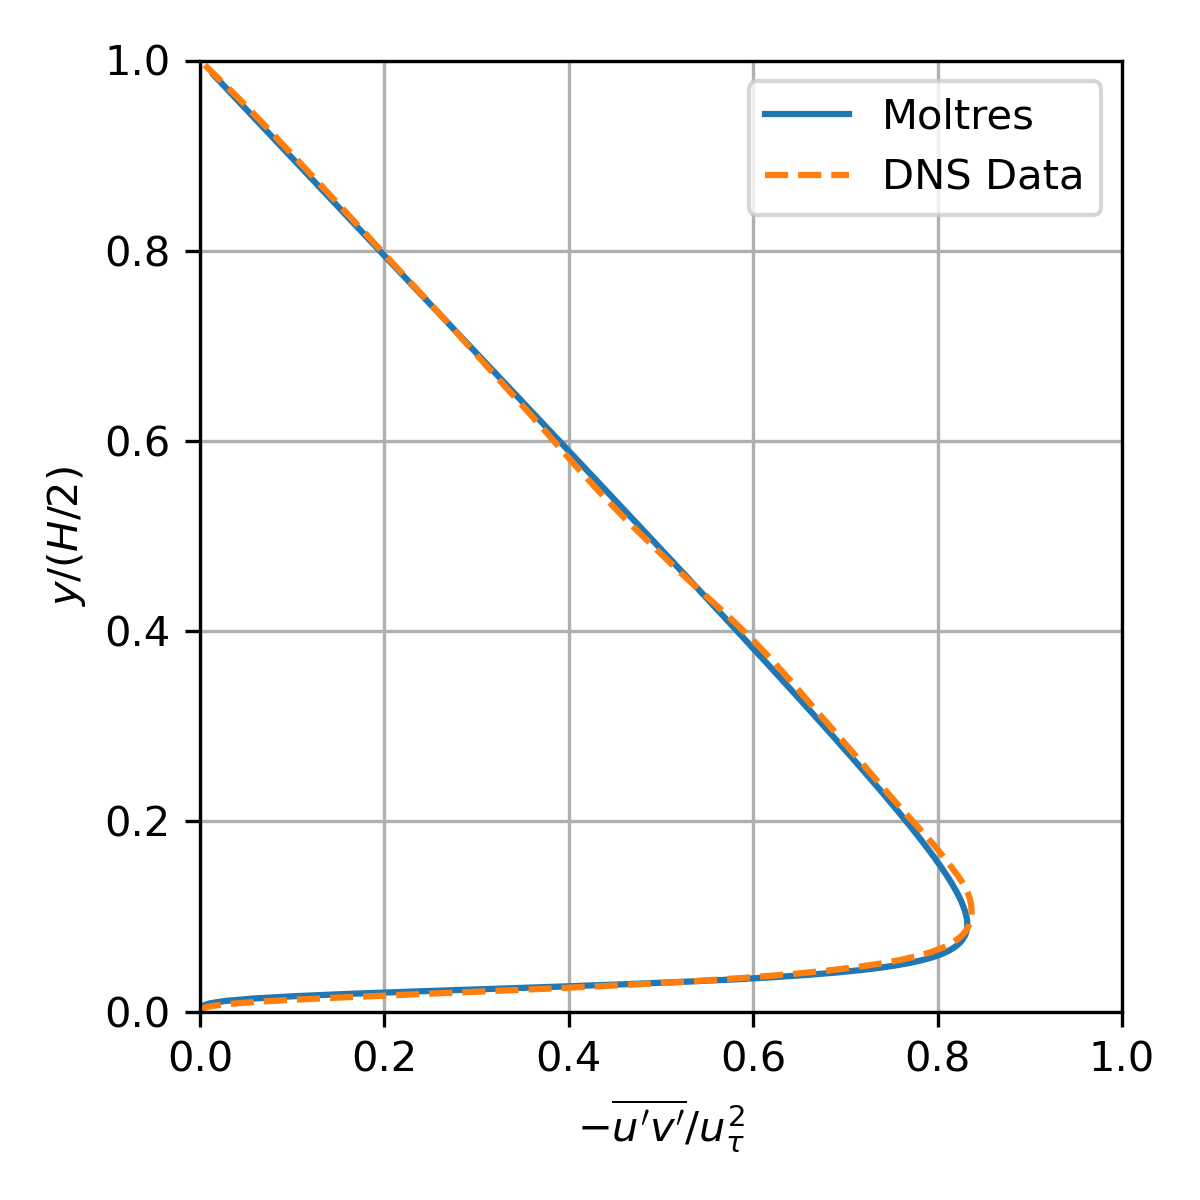
\includegraphics[width=\columnwidth]{channel_stress}
      \caption{Normalized stress distribution across the channel.}
      \label{fig:channel-stress}
    \end{subfigure}
    \caption{Comparison of turbulent channel flow results at Re$_\tau\approx395$ against reference
    \gls{DNS} results \cite{moser_direct_1999}.}
    \label{fig:channel-verification}
  \end{figure}
  \vspace{.1cm}

  $\Rightarrow$ The Moltres Spalart-Allmaras model results are consistent with reference DNS channel flow data.
\end{frame}

\begin{frame}
  \frametitle{Turbulent Pipe Flow Validation Test Results}
  \begin{figure}[htb]
    \centering
    \begin{subfigure}[b]{0.32\columnwidth}
      \centering
      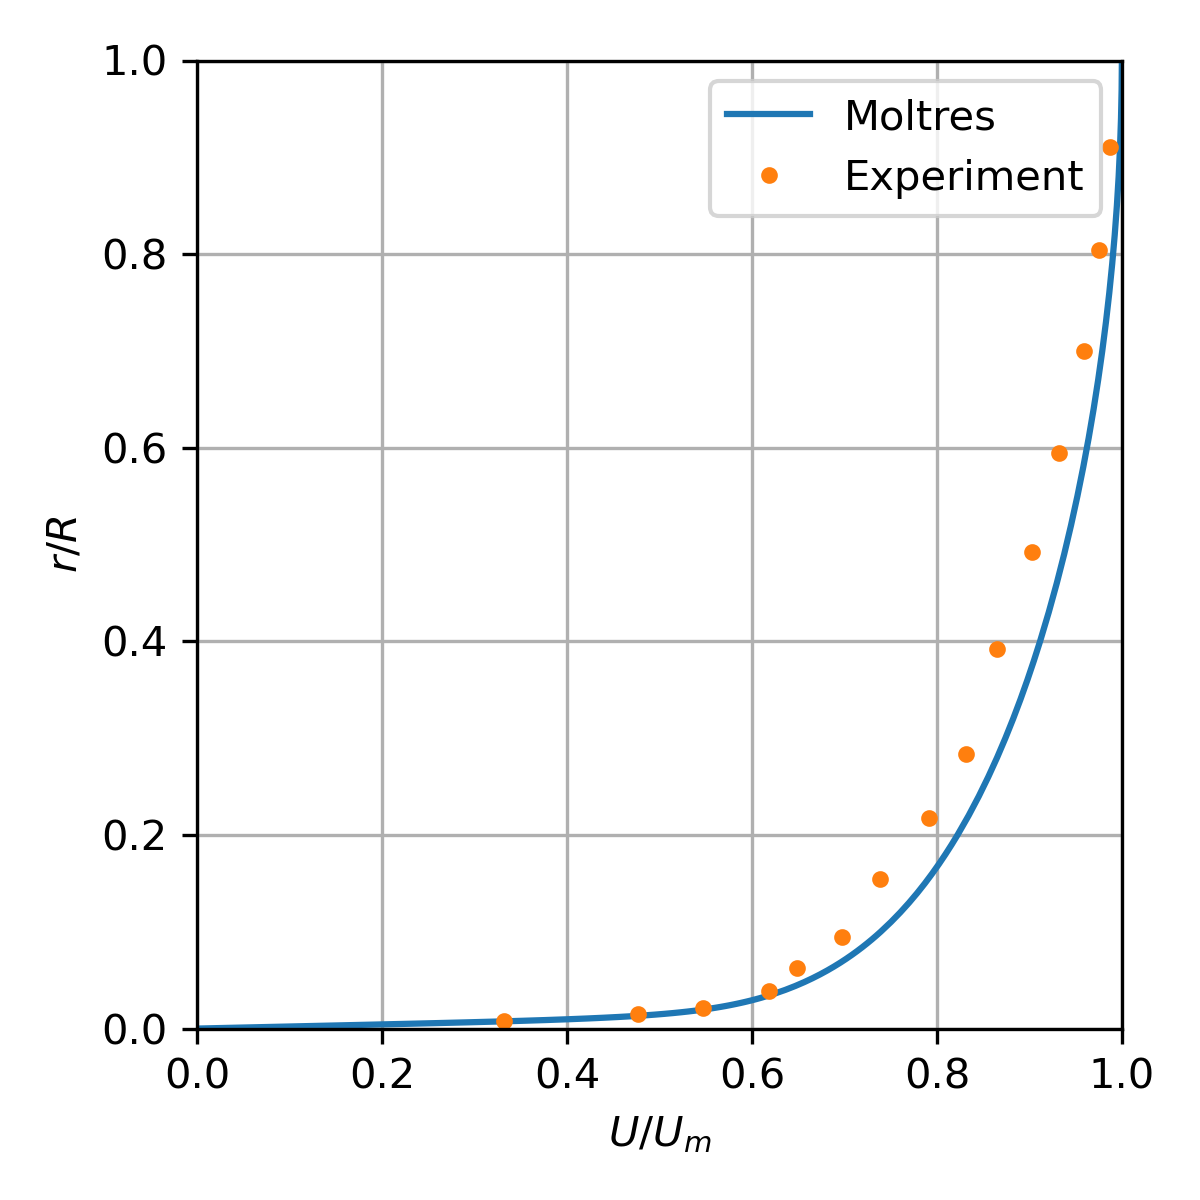
\includegraphics[width=\columnwidth]{pipe_vel}
      \caption{Normalized velocity distribution across the pipe.}
      \label{fig:pipe-vel}
    \end{subfigure}
    \hfill
    \begin{subfigure}[b]{0.32\columnwidth}
      \centering
      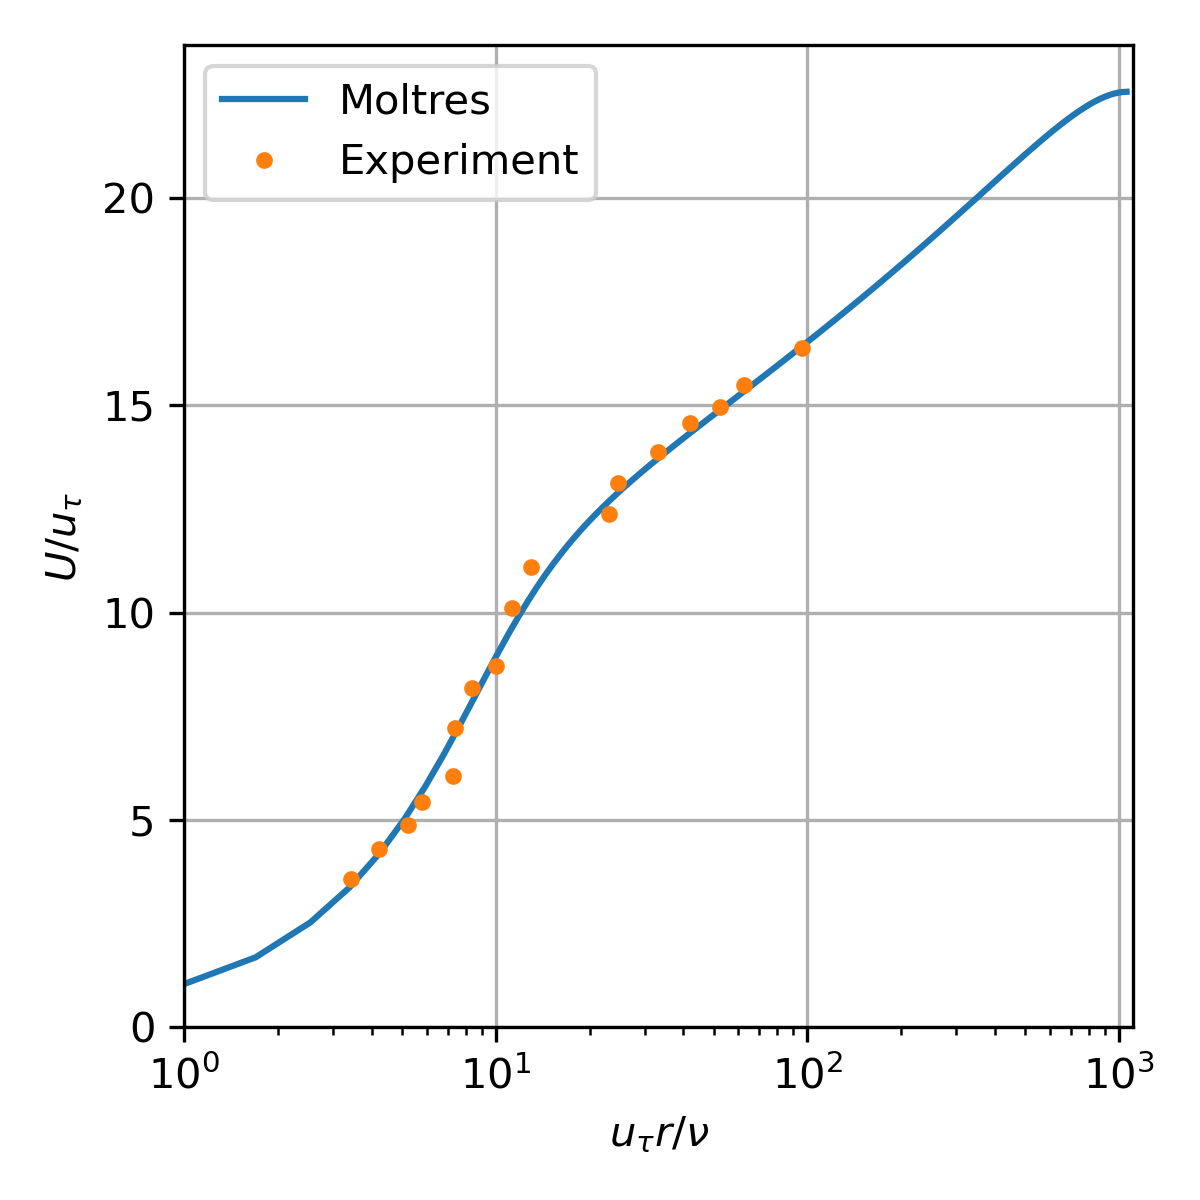
\includegraphics[width=\columnwidth]{pipe_nondim}
      \caption{Dimensionless velocity vs.\ dimensionless wall distance}
      \label{fig:pipe-nondim}
    \end{subfigure}
    \begin{subfigure}[b]{0.32\columnwidth}
      \centering
      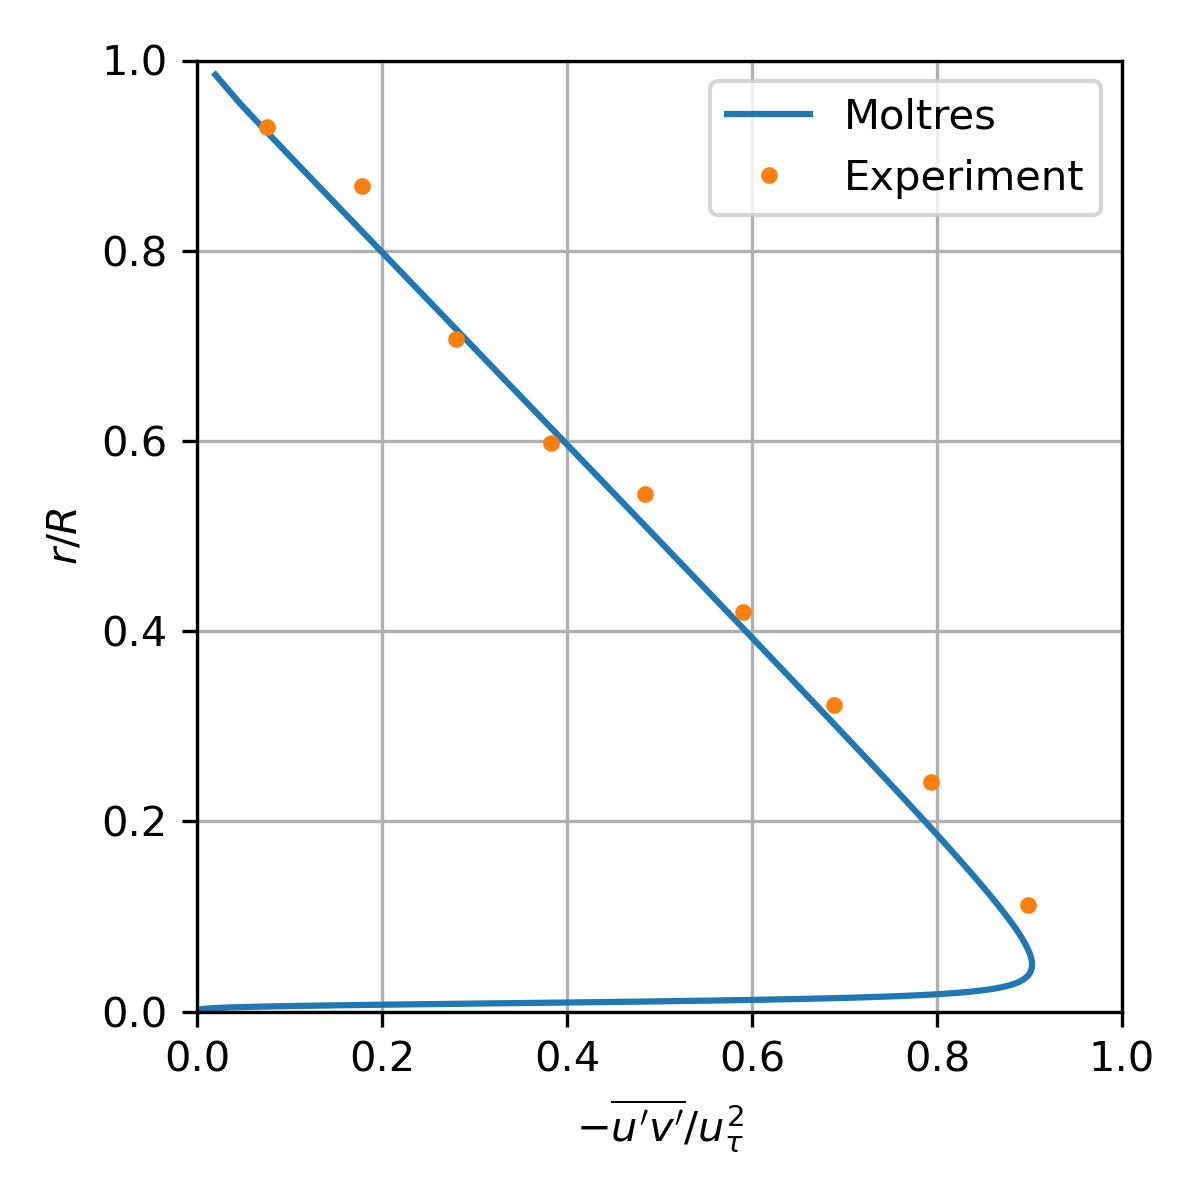
\includegraphics[width=\columnwidth]{pipe_stress}
      \caption{Normalized turbulent shear stress across the pipe.}
      \label{fig:pipe-stress}
    \end{subfigure}
    \caption{Comparison of turbulent pipe flow results at Re $\approx 40000$ against reference
    experimental data \cite{laufer_structure_1954}.}
    \label{fig:pipe-verification}
  \end{figure}
  \vspace{.1cm}

  $\Rightarrow$ The Moltres Spalart-Allmaras model results are consistent with reference experimental pipe flow data.
\end{frame}

\begin{frame}
  \frametitle{Backward-Facing Step Flow Validation Test Setup}
  \begin{columns}
    \column{5.5cm}
    \begin{figure}[h]
      \centering
      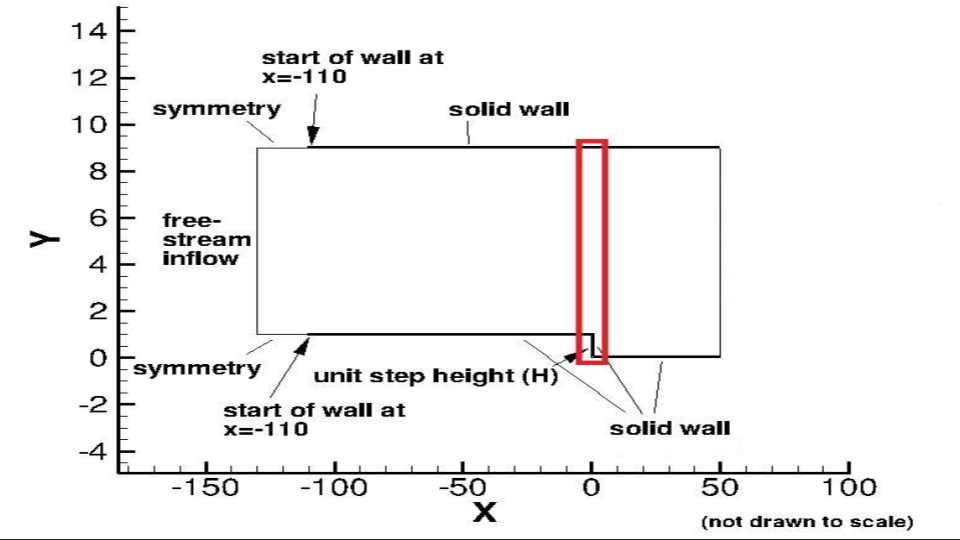
\includegraphics[width=\columnwidth]{backstep-geom-pres}
      \caption{Backward step geometry for the turbulent BFS flow verification test. The red box indicates
      the region shown by the close-up view in Figure \ref{fig:bfs-mesh}.}
      \label{fig:backstep-geom}
    \end{figure}
    \column{5.5cm}
    \begin{figure}[h]
      \centering
      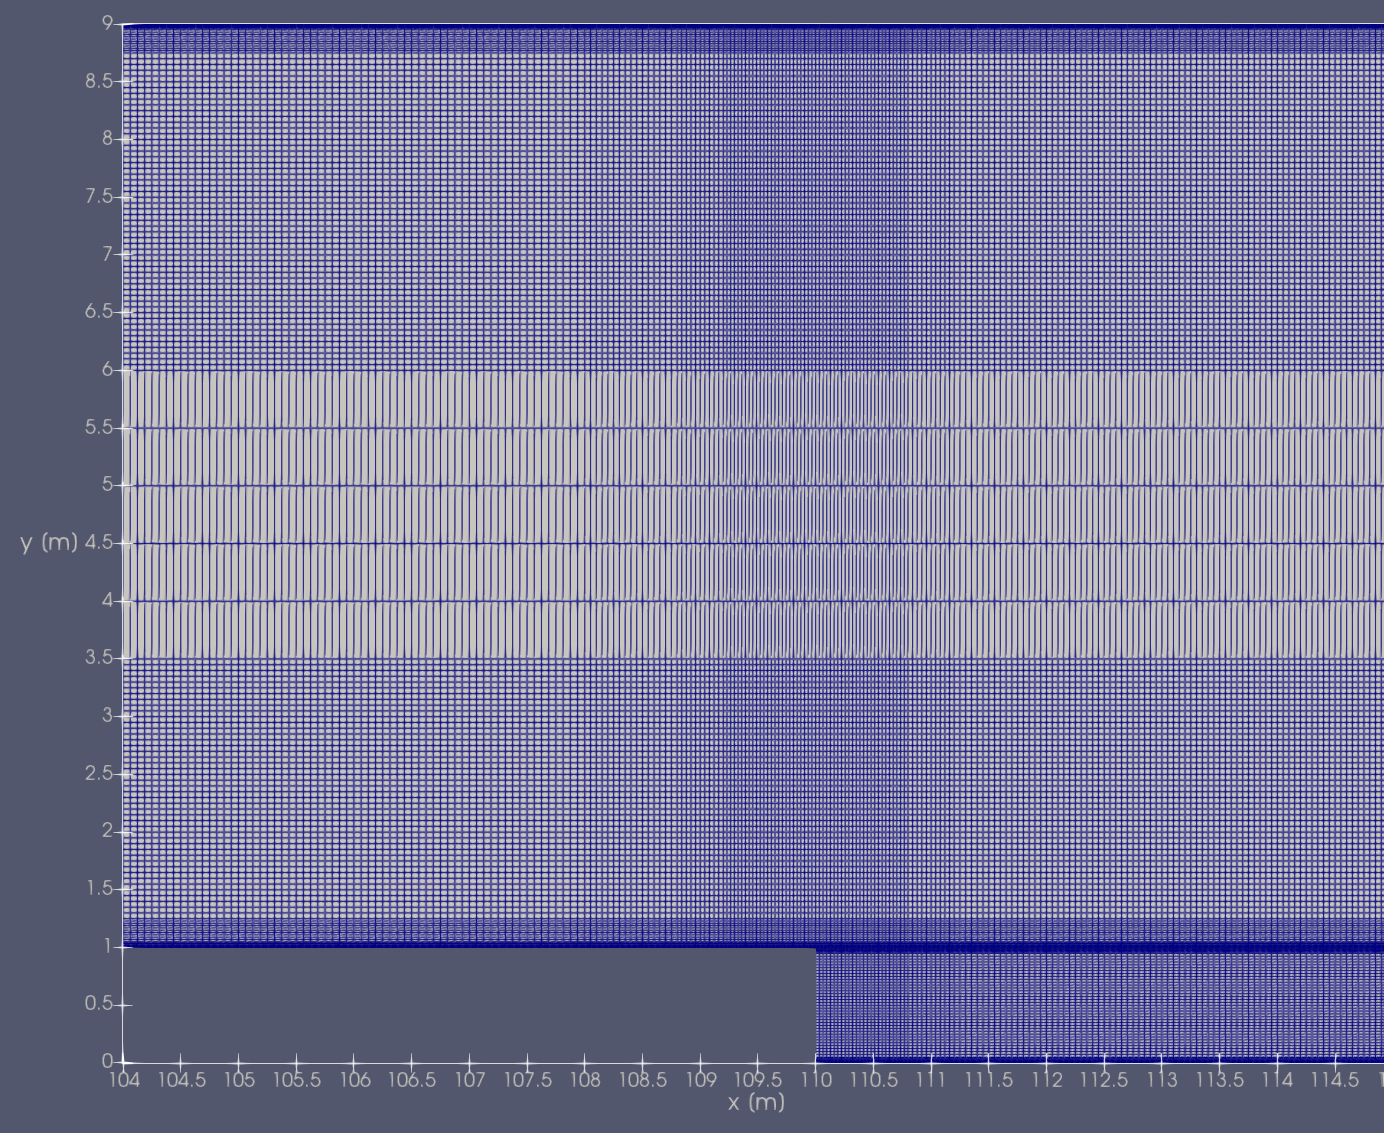
\includegraphics[width=\columnwidth]{bfs_mesh}
      \caption{Close-up view of the mesh for the BFS flow test. The step is situated at $x=110$ m
      with a height of $H=1$ m.}
      \label{fig:bfs-mesh}
    \end{figure}
  \end{columns}
\end{frame}

\begin{frame}
  \frametitle{Backward-Facing Step Flow Validation Test Results}
  \begin{columns}
    \column{5.5cm}
    \begin{figure}[htb!]
      \centering
      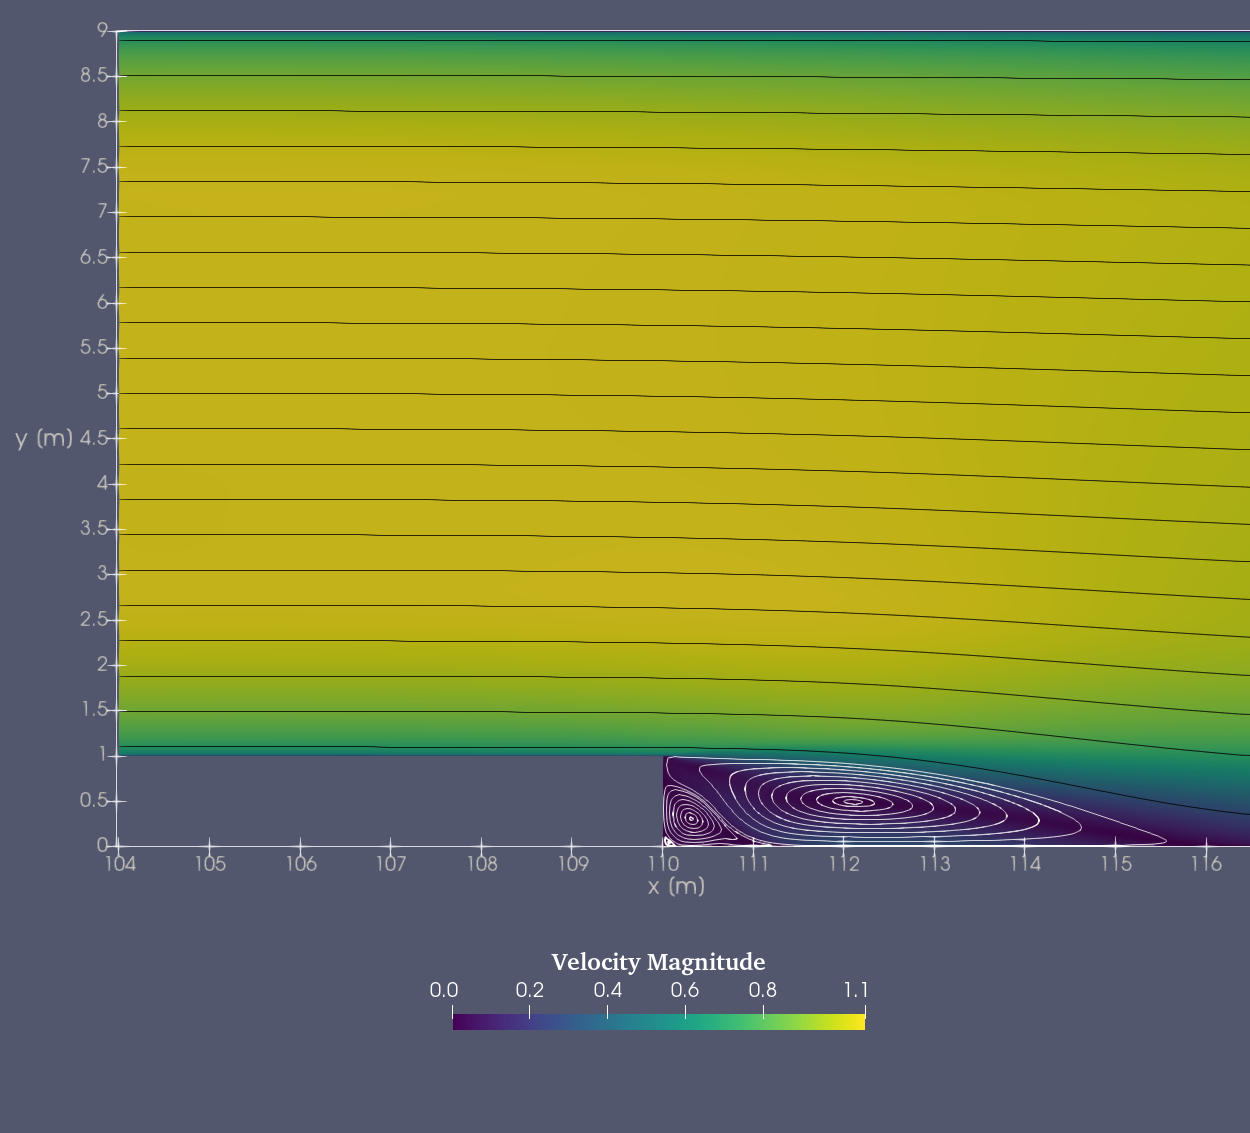
\includegraphics[width=\columnwidth]{bfs}
      \caption{Velocity magnitude distribution and streamlines around the backward-facing step. The
      streamlines illustrate the primary and secondary recirculation zones.}
      \label{fig:bfs}
    \end{figure}
    \column{5.5cm}
    \begin{table}[htb]
      \centering
      \scriptsize
      \caption{BFS flow reattachment length estimates normalized by step height $H$.}
      \begin{tabular}{l S[table-format=1.2(2)]}
        \toprule
        Source & {Reattachment length [-]} \\
        \midrule
        Experimental data & 6.26(10) \\
        CFL3D & 6.1 \\
        Moltres & 6.36 \\
        \bottomrule
      \end{tabular}
      \label{table:bfs-reattach}
    \end{table}
    \vspace{.1cm}

    $\Rightarrow$ Moltres is consistent with experimental data (within uncertainty range) while CFL3D
    falls outside the uncertainty range.
  \end{columns}
\end{frame}

\begin{frame}
  \frametitle{Backward-Facing Step Flow Validation Test Results}
  \begin{columns}
    \column{11.5cm}
    \begin{figure}[htb]
      \centering
      \begin{subfigure}[t]{0.32\columnwidth}
        \centering
        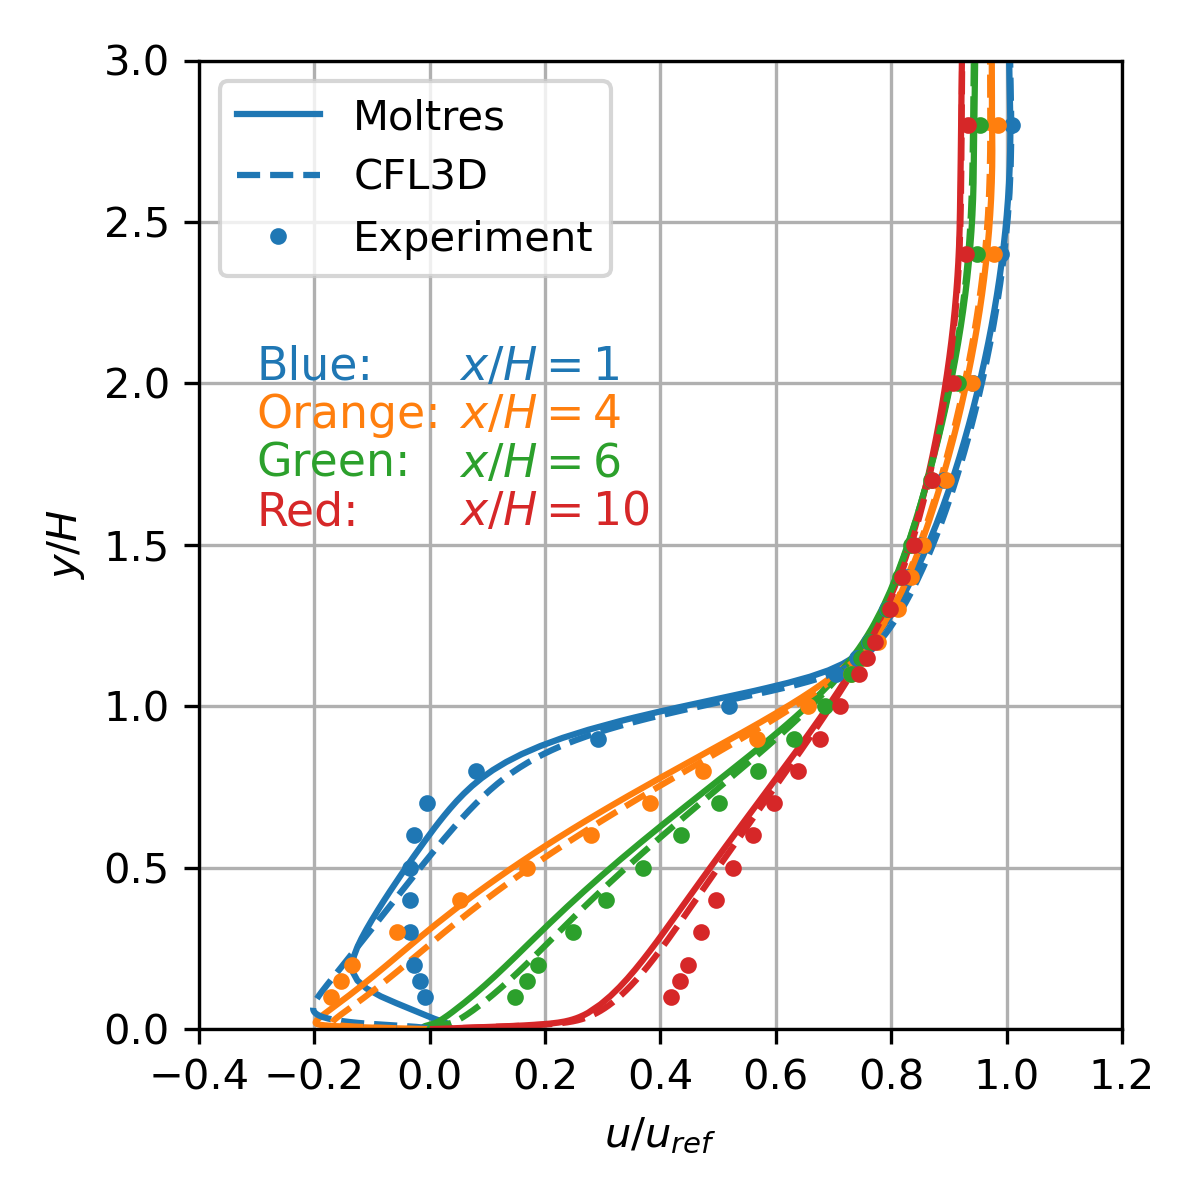
\includegraphics[width=\columnwidth]{bfs_downstream_vel}
        \caption{Normalized velocity distributions downstream of step.}
        \label{fig:bfs-downstream}
      \end{subfigure} %\hfill \\
      \begin{subfigure}[t]{0.32\columnwidth}
        \centering
        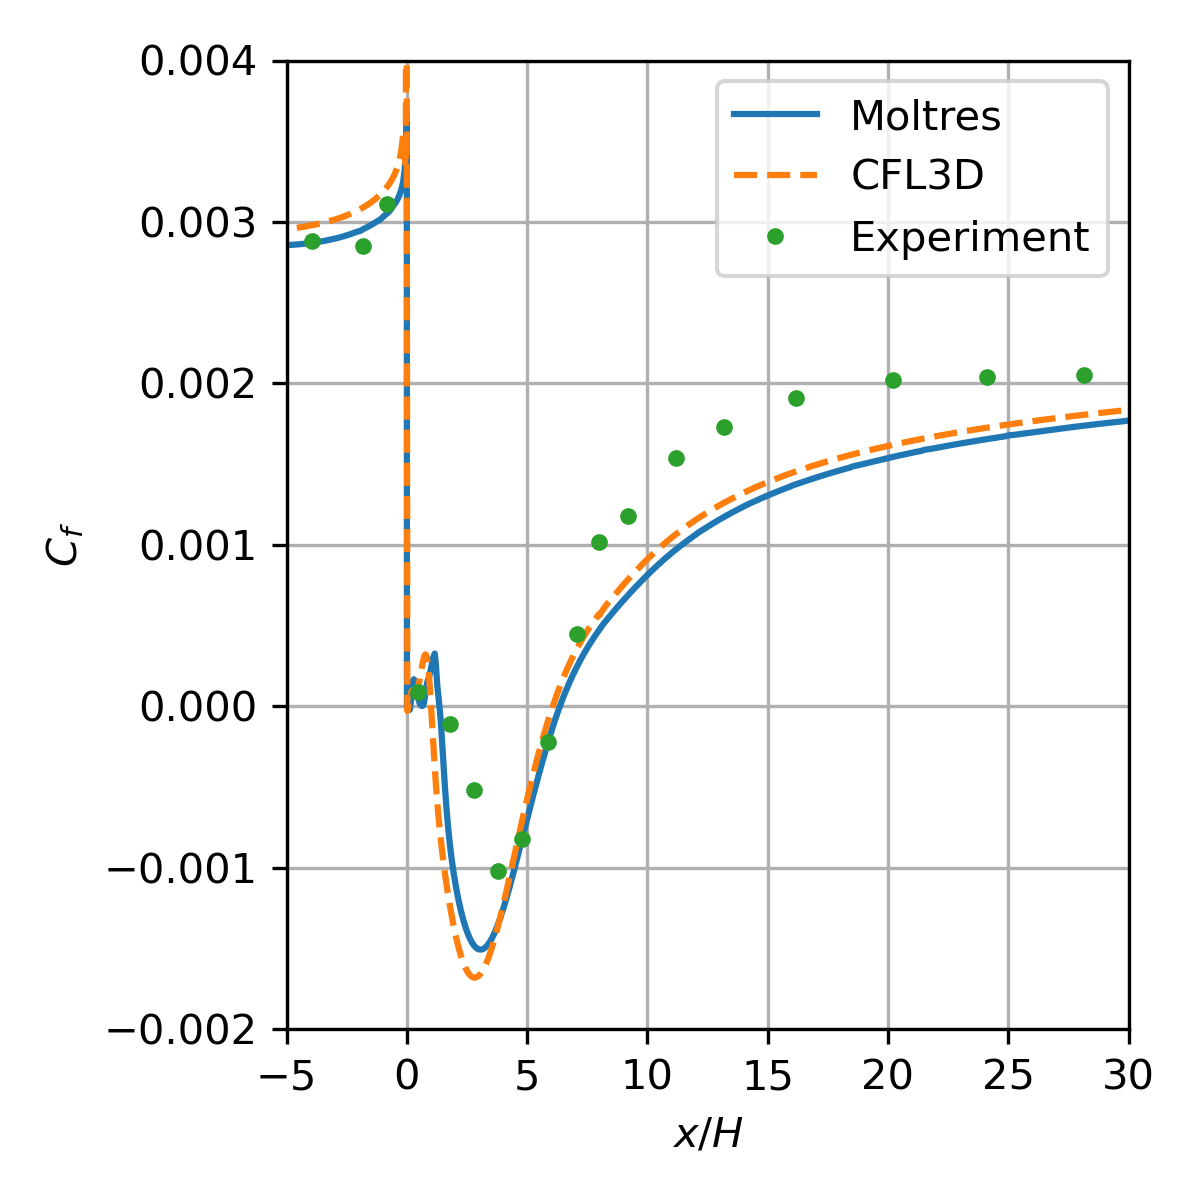
\includegraphics[width=\columnwidth]{bfs_cf}
        \caption{Skin friction coefficient along the bottom wall.}
        \label{fig:bfs-cf}
      \end{subfigure}
      \begin{subfigure}[t]{0.32\columnwidth}
        \centering
        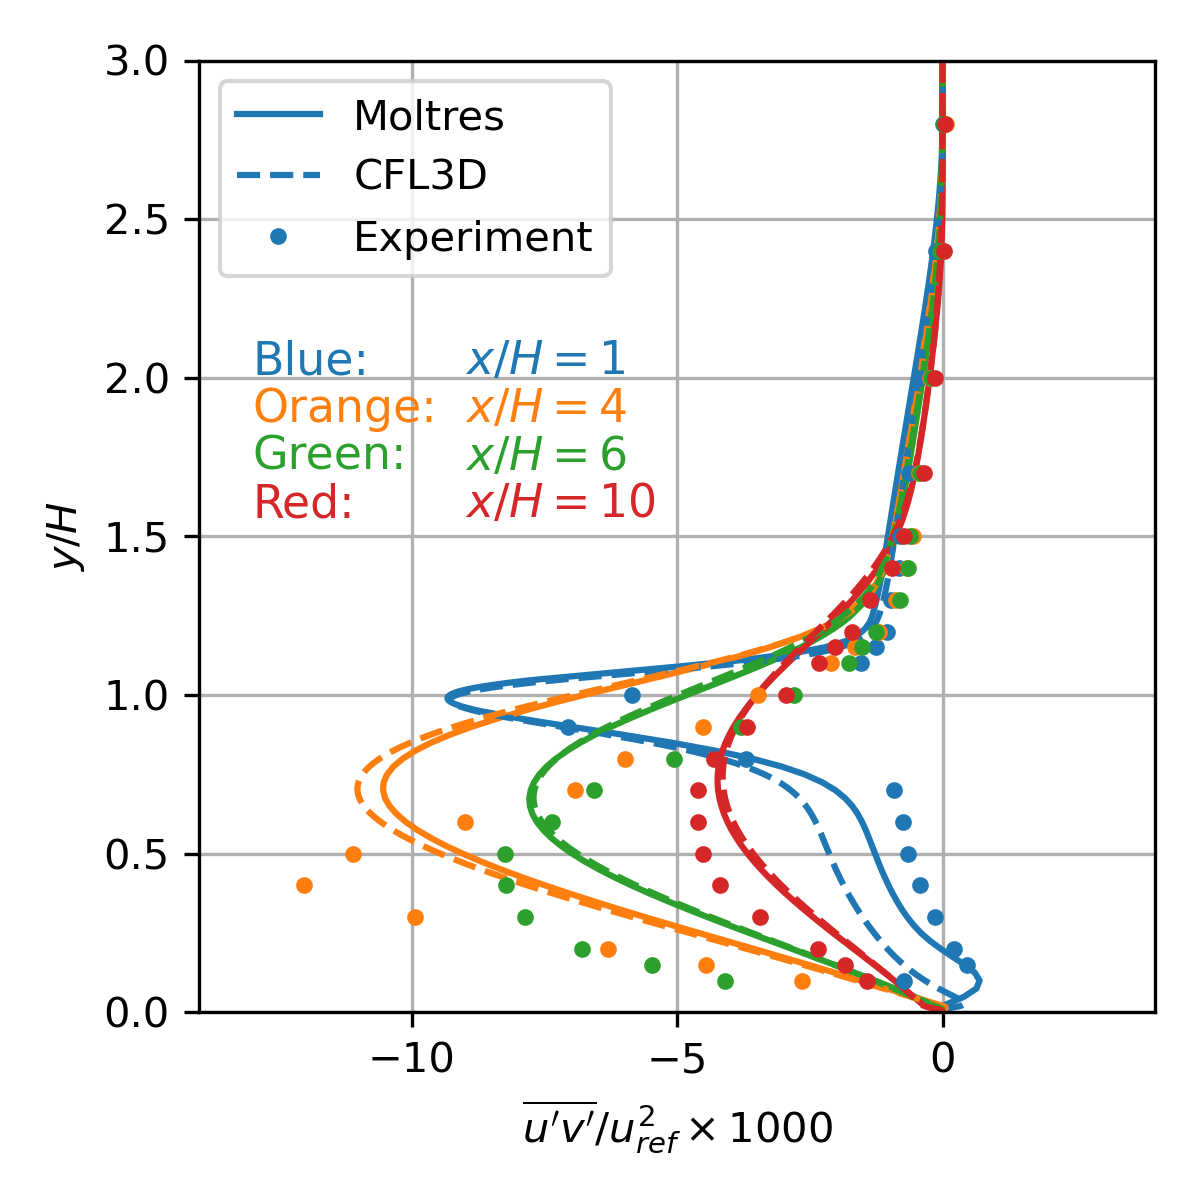
\includegraphics[width=\columnwidth]{bfs_stress}
        \caption{Normalized turbulent shear stress downstream
        of step.}
        \label{fig:bfs-stress}
      \end{subfigure}
      \caption{Comparison of backward facing step flow results against reference
      experimental data and computational data from CFL3D. $x/H$ values are normalized horizontal
      distances relative to the step.}
      \label{fig:bfs-plots}
    \end{figure}
  \end{columns}
  \begin{itemize}
    \item Minor discrepancies between numerical and experimental data typical of RANS-based turbulence models.
    \item Moltres provides more accurate measurements along $x/H=1$ than CFL3D.
  \end{itemize}
\end{frame}

\begin{frame}
  \frametitle{Spalart-Allmaras Turbulence Model in Moltres}
  \begin{block}{\textbf{Spalart-Allmaras Model V\&V Test Summary}}
    \begin{itemize}
      \item Good agreement between Moltres and reference solutions in the turbulent channel and pipe
        flow tests.
      \item Good agreement between Moltres and CFL3D in the backward-facing step flow test.
      \item Some discrepancy between Moltres and experimental data in the backward-facing step flow
        test, but Moltres performed better than CFL3D at predicting flow reattachment length and
        velocity/stress distributions along $x/H=1$.
    \end{itemize}
  \end{block}
\end{frame}
